\section{Supporting qualification evidence}
\label{app:res-evidence}
This appendix preserves the detail needed to interpret the main qualification tests without repeating the Design's subsystem derivations. The source package contains the original v6 measurement archive, the reviewed aggregate records and the scripts that generate the revised tables and figures. Newly computed analyses are identified separately from the original measurements. No physical measurement is generated by a plotting script.

\subsection{Evaluated checkpoints and populations}
The selected demonstration reader is the library-trained joint reader, as confirmed by the author. The numerical scratch reader is a comparison model. The selected writer model is the library-trained eleven-writer 0.17 model. Table~\ref{tab:app-checkpoints} records hash prefixes; the evidence manifest retains the full SHA-256 values. A filename alone is insufficient because the archived reader study identified two different files named \texttt{scratch\_best}.

\begin{table}[!htbp]\centering\small
\begin{tabular}{lll}\toprule
\textbf{Role} & \textbf{Checkpoint identifier} & \textbf{SHA-256 prefix}\\\midrule
Selected reader & joint\_best & \texttt{336802d535992323}\\
Comparison reader & evaluated scratch\_best & \texttt{2add315ded078de5}\\
Selected writer & 11\_pw170 & \texttt{1884fb86467538eb}\\
Comparison writer & 11w\_pw170\_scratch & \texttt{b23a709a30144f67}\\\bottomrule
\end{tabular}
\caption{Identities of the measured model files.}\label{tab:app-checkpoints}\end{table}

The numerical-writer training excerpt supplied by the author records 1\,031 training lines and 155 validation lines, 0.17 normalisation, a 50-epoch budget and a best displayed validation accuracy of 0.968 by epoch 41. The retained excerpt continues through epoch 47 and does not document a completed epoch 50. Its later common-set score is measured on 156 re-extracted validation lines; the different population is retained rather than silently equated with training validation. The numerical-reader excerpt records 6\,481 public training lines, 569 personal training lines, 976 public validation lines and 100 personal validation lines, and a resume from an existing checkpoint. These are training-history records, while QT~2 evaluates saved weights directly.

An additional inventory reads each selected stored profile and verifies nonempty glyph mappings. The numbers of distinct character keys are 42, 38, 37, 36, 40 and 41 for the six database writers, and 56, 42, 43, 42 and 58 for A, B, O, T and Y. All eleven names agree with the selected writer checkpoint. The full source paths and content hashes are preserved in \texttt{ResultsEvidence/profile\_inventory.json}. These counts establish stored mappings; they do not imply equal coverage of every character in the reader alphabet.

\subsection{Physical reproduction by writer}
\begin{table}[!htbp]\centering\small
\begin{tabular}{lrrrr}\toprule
\textbf{Writer} & \textbf{Lines} & \textbf{Character / \%} & \textbf{Writer / \%} & \textbf{Word match / \%}\\\midrule
Y & 13 & 97.01 & 92.31 & 74.16\\
150 & 13 & 96.75 & 53.85 & 76.40\\
O & 16 & 94.25 & 100.00 & 58.51\\
B & 16 & 93.11 & 93.75 & 68.24\\
384 & 16 & 86.93 & 87.50 & 43.18\\
552 & 15 & 86.17 & 80.00 & 48.39\\
152 & 15 & 85.74 & 80.00 & 49.44\\
A & 27 & 77.29 & 100.00 & 18.09\\
153 & 19 & 75.72 & 57.89 & 31.46\\
588 & 18 & 73.19 & 94.44 & 22.99\\
T & 16 & 60.97 & 100.00 & 13.41\\
\bottomrule\end{tabular}
\caption{Full per-writer reproduction results on 184 labelled lines. Word match uses equal word positions and is not one minus word edit error rate.}\label{tab:app-r1-writers}
\end{table}

The paired read-back study contains 184 transcript-bearing lines. A separate model comparison contains 185 writer-labelled crops, including one crop with no corresponding transcript line. It can support a writer-prediction comparison, but that extra crop is not inserted into a character score. The model-comparison pooled groups are writers, not a claim that only eleven physical sheets were drawn.

\subsection{New geometric style comparison on physical pages}
\label{app:res-physical-style}
The new analysis applies the archived descriptor definitions with the current segmentation primitives to 156 original reference lines and 184 physical-output lines. The original population consists of the same six held-out database pages and 100 seeded photographed reference lines used for writer evaluation. The physical population comprises all fourteen robot pages after the recorded orientation convention. Each page's crop count agrees with its transcript-bearing records, and every line returns usable descriptors. All eleven writers are retained.

Each line is binarised, its body band estimated and its image resized toward a 28-pixel body height before the descriptors are evaluated. The same procedure is applied to both domains. Writer means give equal weight to available lines for each feature, and the pooled correlation gives equal weight to writers and selected features. Word-gap values are absent where no qualifying gap exists: 155/156 original and 180/184 physical lines have a value; the other descriptors are available for every line. All eleven writer means remain usable. The within-domain variant separately standardises each feature in each domain; the absolute variant uses original-domain means and standard deviations for both. Source images, the personal-crop cache, scripts and full measurements are recorded by hash. The raw outputs are in \texttt{ResultsEvidence/physical\_style/results.json}.

The per-feature correlations are slant 0.9911; stroke width 0.7986; ink density 0.7392; word gap 0.4861; components per word 0.6688; character width 0.7978; ascender extent 0.8173; descender extent 0.5394; and extent ratio 0.5762. Figure~\ref{fig:app-physical-style} shows the actual writer means. The 10\,000-repeat writer-resampling range for the seven-feature within-domain coefficient is 0.5555--0.8272, using seed 23539195. It is a sensitivity range over this writer set. This retrospective comparison does not use identical sentences between domains and should not be interpreted as a controlled perceptual-equivalence experiment.
\begin{figure}[!htbp]\centering
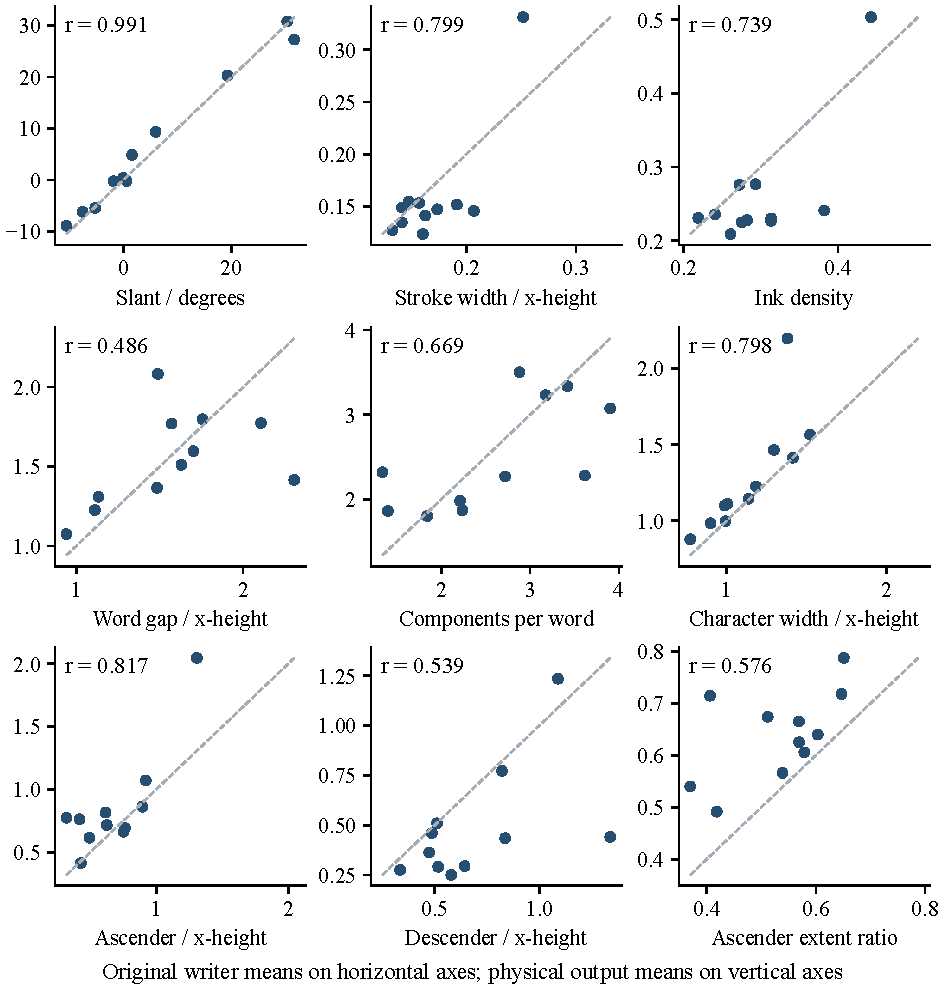
\includegraphics[width=0.99\linewidth]{Figures/results_physical_style_scatter.pdf}
\caption{New physical-to-original style descriptors across eleven writers. Each point is one writer mean. Dashed lines indicate equal values; correlation can remain high even when magnitudes differ.}\label{fig:app-physical-style}\end{figure}

\subsection{Archived geometric style study}
\label{app:res-style}
The archived study covers writers 150, 151, 152, 153, 384, 551, 552, 588, B and Y. There are six synthetic lines per writer, sixty in total, compared with 123 original reference lines marked as excluded from profile building. This earlier ten-writer set differs from the final eleven-writer evaluation. The study is retained to explain geometric behaviour of the method; it is not relabelled as a measurement of final physical pages.

Nine deterministic descriptors measure slant, normalised stroke width, ink density, word gap, components per word, character width, ascender extent, descender extent and the ascender-to-total-extent ratio. Seven shape descriptors omit stroke width and ink density. The within-domain pooled correlation first standardises each feature across writers separately in the real and synthetic domains, then correlates the flattened arrays. It is therefore insensitive to a uniform offset or scale difference between those domains. The alternative absolute variant standardises both arrays using the real-domain mean and standard deviation. This distinction matters when interpreting preservation of magnitude rather than writer ordering.

\begin{table}[!htbp]\centering\small
\begin{tabular}{lrr}\toprule
\textbf{Feature set} & \textbf{Separate-domain standardisation} & \textbf{Real-domain standardisation}\\\midrule
Nine features & 0.7013 & 0.5994\\
Seven shape features & 0.7142 & 0.6711\\\bottomrule
\end{tabular}
\caption{Archived synthetic-to-original pooled correlations against the profile-held-out reference. The 0.714 value is the seven-shape-feature variant.}\label{tab:app-style-variants}\end{table}

The per-feature coefficients are 0.9964 for slant, 0.6315 for stroke width, 0.6802 for ink density, 0.6050 for word gap, 0.8323 for components per word, 0.9358 for character width, 0.9735 for ascender extent, 0.1480 for descender extent and 0.5085 for the extent ratio. Correlation describes variation across writers; it does not prove pointwise agreement of all letter shapes. The recorded 2\,000 writer-resample interval for the seven-feature within-domain result is 0.6118--0.8586.

The archived overlay experiment uses thirty source texts across those ten writers. With x-height normalisation, mean matched chamfer distance is 0.6302, mean mismatched distance is 1.3868, their ratio is 2.2007 and the recorded AUC is 0.7074. When the archive also applies its width-normalisation variant, AUC is 0.4630. Thus the favourable separation depends on the chosen normalisation; an AUC above 0.5 in one variant must not be presented as universal writer fidelity. These remain software comparisons, without a new independent human panel.

\subsection{Timing selection and optimisation scope}
\label{app:res-speed}
QT~3 uses a deliberately checkable completion boundary. The earlier archive retained 36 records after deduplication and a drawing-rate filter. The revised primary count uses 25 positive-character console records with explicit program-end evidence. The original 36-record aggregation remains in the preserved provenance document. A rate threshold alone does not establish completion: a job stopped after substantial drawing can exceed that threshold. This change does not alter the observed worst 3.875~s per character. A terminal marker confirms the interpreter finished, while geometry and content remain separate qualification questions.

The 500- and 982-character counts for QT~4 are the counts printed in the timer record. A final repeat should retain independent transcript lengths and an acquisition-to-output timing boundary. The two current overruns are large, so no inferred sub-second camera transfer time is added to create a favourable pass.

\begin{table}[!htbp]\centering\small
\begin{tabularx}{\linewidth}{lX}\toprule
\textbf{Comparison} & \textbf{Measured outcome and scope}\\\midrule
Sequential NumPy vs batched library networks & 359.8~s vs 130.3~s over fourteen stored pages on the development host; factor 2.76. Both backend and batching change. Reader text is identical; writer-label equivalence is not inferred from that fact.\\[4pt]
Full vs half linear image resolution & 4.37-fold recorded image-stage factor on comparable successful page pairs, with 247 vs 182 detected lines. Zero of twelve comparable pages retain line count; two of fourteen reduced pages fail segmentation.\\[4pt]
Projected network-only replacement & Applying 2.76 to ODROID network stages, with image stages unchanged, gives approximately 27.05~s and 30.82~s. Neither is an observed ODROID result or a total-time pass.\\[4pt]
Projected combined replacement & Applying both host factors gives approximately 14.61~s and 17.86~s. The second is numerically below its allowance, but the image reduction changes the output and the timing is transferred between hosts. It is not accepted as R4 compliance.\\\bottomrule
\end{tabularx}
\caption{Acceleration evidence and the boundary between a measured comparison and a projected compliant configuration.}\label{tab:app-acceleration}\end{table}

The G-code study of the same 378-character paragraph yields pen-down path lengths from 2\,015.4 to 3\,942.8~mm and recorded pen-state counts from 544 to 1\,188 across eleven profiles. These are arithmetic properties of generated paths. They demonstrate profile-dependent geometry and help explain timing variation; they are not independent proof of similarity to genuine handwriting, and their values can still be affected by the candidate-selection process.

\subsection{Planned repeated-word and physical overlay record}
\label{app:res-overlay}
\begin{figure}[!htbp]\centering
\designasset{results-repeated-word-overlay.pdf}{0.90}{Two executions of the same word using fixed glyph choices, seed, size and layout, shown against one coordinate reference. Include the original scans, scale, point-registration method, maximum measured displacement, repeated-draw count and measurement uncertainty. This is a pending measurement, not a predicted passing result.}
\caption{Reserved repeated-word overlay required to extend the gantry qualification.}\label{fig:res-overlay-pending}\end{figure}
The overlay should keep machine placement visible: unconstrained image translation or warping would hide the absolute-position error being tested. A separate original-versus-reproduced handwriting illustration should state whether the text, scale and baseline are matched, and distinguish qualitative resemblance from a measured geometric metric.

\subsection{Cost, consent and final records}
The photographed ledger supplied by the author is retained as evidence. The present build estimate is approximately R4\,000, with a borrowed ODROID entered at zero purchase cost. The later listed clipboard (R90), paper (R130), gel pen (R30) and estimated training electricity (R500) total R750. The final account must establish which are already included in the estimate; no exact total is produced by adding overlapping entries. Replacement value and estimated operating costs should be distinguished from actual purchased parts.

Signed consent forms are held by the author for the five personal contributors. The report records that fact without reproducing signatures. A redacted consent template may be supplied where institutionally required. The institutional clearance or exemption reference, printed-part material, caliper identification and measured lighting record remain author-supplied completion items.

\subsection{Supporting timing and dimensional figures}
\begin{figure}[!htbp]\centering
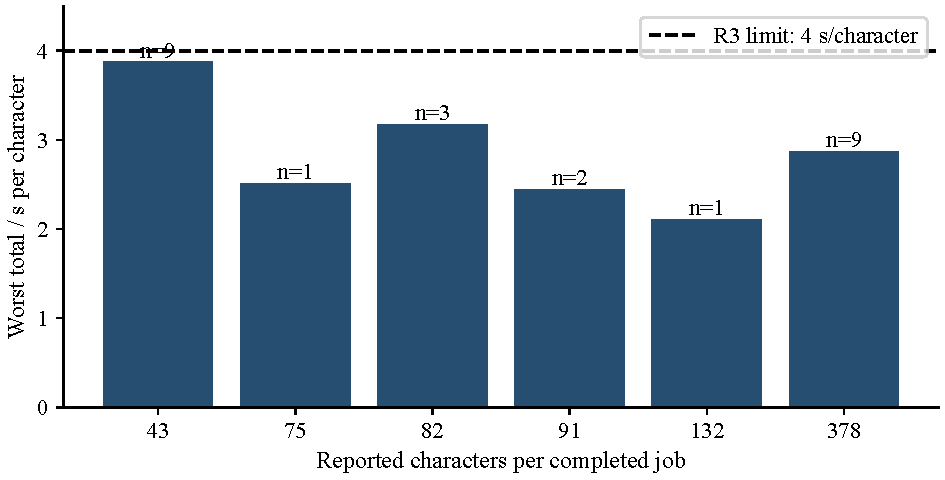
\includegraphics[width=0.98\linewidth]{Figures/results_r3_confirmed.pdf}
\caption{Worst recorded generation-plus-drawing time at each tested length, using only explicitly completed jobs. Labels state the number of records. The timing result applies to these recorded jobs and does not imply identical quality for every writer.}
\label{fig:res-r3}\end{figure}
\begin{figure}[!htbp]\centering
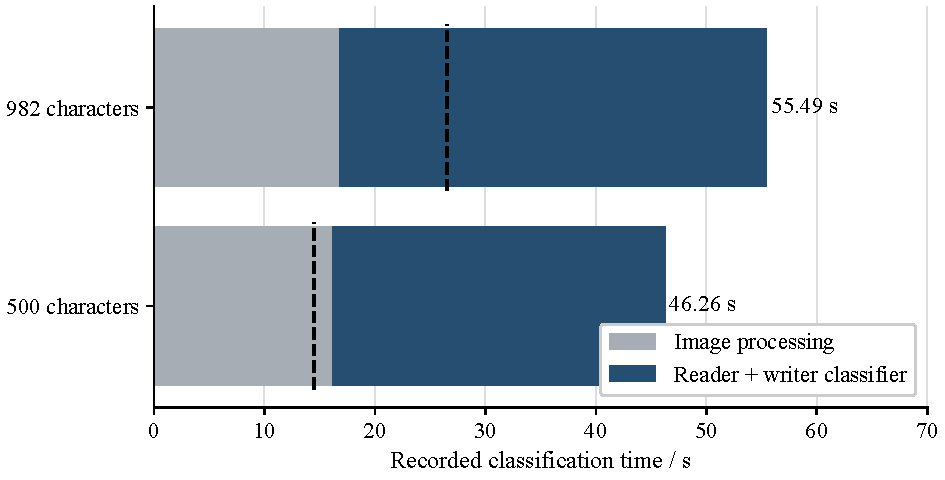
\includegraphics[width=0.98\linewidth]{Figures/results_r4_stages.pdf}
\caption{Recorded ODROID classification time split into image and network stages. Dashed markers show the complete R4 allowance at each logged character count. Both measured totals exceed their allowance.}
\label{fig:res-r4}\end{figure}
\begin{figure}[!htbp]\centering
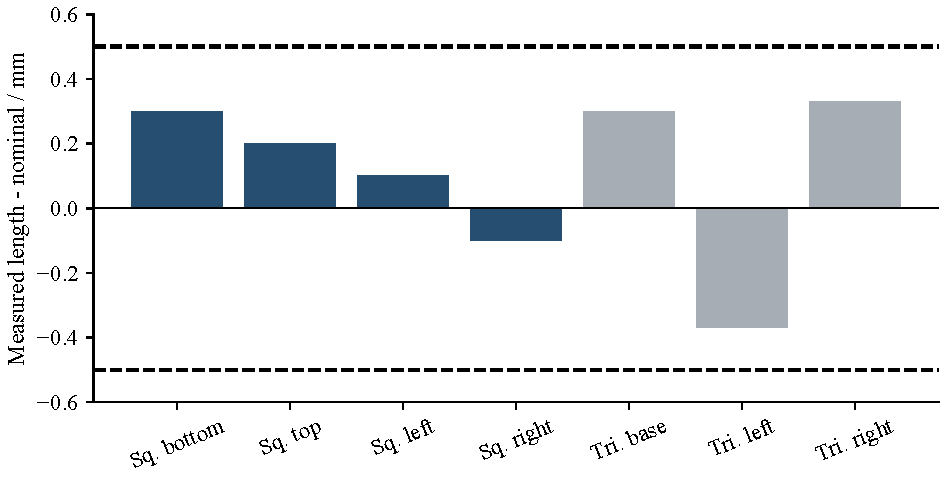
\includegraphics[width=0.98\linewidth]{Figures/results_geometry_errors.pdf}
\caption{Signed dimensional differences for one square and one triangle. Dashed lines are the 0.5~mm reference. Being inside those lines is a feature-length observation, not an absolute coordinate-error bound over the bed.}
\label{fig:res-geometry}\end{figure}
